\chapter{Introdução}

Adicionar motivação pelo tema - Por que resolver um problema ligado aos portadores de necessidades? (Obs - não é problematizar)

\section{O Problema}

O desenvolvimento da opção mais básica de mobilidade para portadores de mobilidade
reduzida, a cadeira de rodas, vem tornando-se cada vez mais estagnada. 
Mesmo com a adaptação do modelo clássico para modelos motorizados, não há, 
fora isso, muitas outras opções de mercado a fim de valorizar o conforto 
e facilitar a vida do usuário e seus familiares. Atualmente, a oferta de 
cadeira de rodas motorizadas com tecnologias semelhantes torna-se cada 
vez mais comum em um cenário onde um alto número de pessoas continua a optar 
por modelos clássicos devido aos altos custos dos modelos presentes no 
mercado internacional. A falta de opções com novas funcionalidades no mercado 
e o alto custo das soluções já existentes tornam o acesso a essas novidades
 cada vez mais restrito.\\
	
Além disso, a ausência de um familiar ou cuidador em certos momentos 
do dia 
dificulta o monitoramento de atividades motoras ou necessidades 
do usuário. 
Com isso em foco, o monitoramento remoto contínuo do usuário 
poderia 
aumentar ainda mais sua liberdade em um ambiente doméstico e, ainda 
assim, 
manter familiares e cuidadores atentos a sinais e alertas e evitando 
possíveis 
acidentes e situações fora do cotidiano.\\
	
O problema, juntamente às suas causas, são representados em um diagrama 
de Causa e Efeito, ou fishbone, conforme Figura \ref{fishbone}.
	
\begin{figure}[h]
    \centering
    \label{fishbone}
    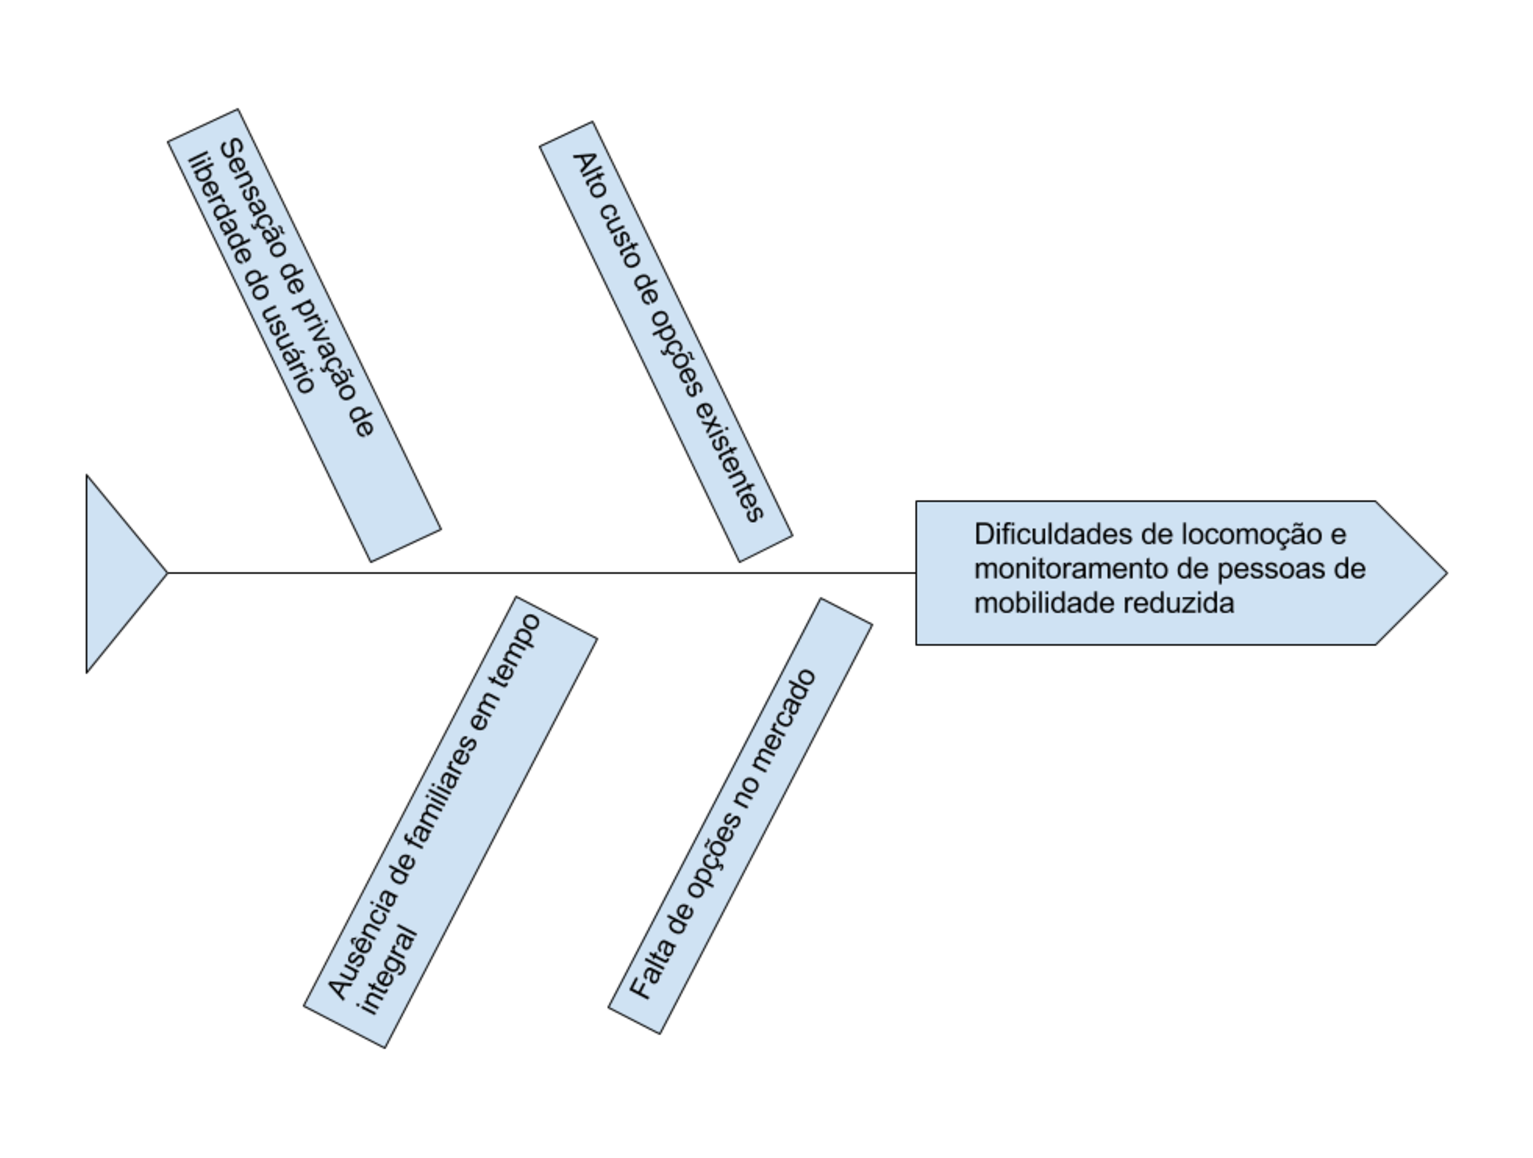
\includegraphics[keepaspectratio=true,scale=0.5]{figuras/fishbone.eps}
    \caption{Diagrama de causa e efeito (\textit{fishbone}) para mapeamento do problema.}
\end{figure}


\section{Estado da Arte}

Dentre as opções para cadeiras de rodas motorizadas acessíveis existentes no mercado,
é comum deparar-se com alternativas para adaptação de cadeiras convencionais,
como por exemplo o sistema \textit{Light Drive} produzido pela empresa britânica, 
com sede em Bristol, \textit{Benoit Solutions}. Este sistema consiste em um \textit{kit}
contendo um baterias, dois motores, uma roda traseira para prevenção de possíveis
acidentes e quedas, e um sistema de controle do tipo \textit{joystick}
para controle de velocidade e direção da cadeira de rodas.\\

Na Figura \ref{ldrive} é possível visualizar os componentes do sistema e
o sistema inserido em uma cadeira de rodas convencional.

\begin{figure}[h]
    \centering
    \label{ldrive}
    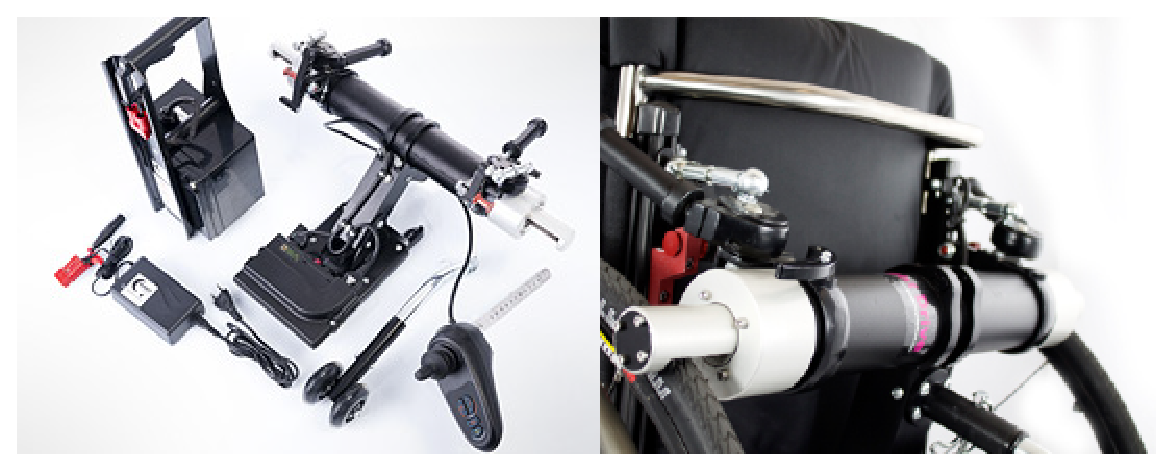
\includegraphics[keepaspectratio=true,scale=0.7]{figuras/ldrive.eps}
    \caption{Sistema de adaptação \textit{Light Drive} da empresa britânica \textit{Benoit Solutions}.}
\end{figure}

O sistema utiliza dois motores de 12V e 100W de potência para a movimentação 
de cadeiras de rodas convencionais, que geralmente possuem pesos de cerca de 16Kg 
e possui um sistema de baterias que pode ser escolhido pelo usuário entre modelos 
de Níquel Metal Hidreto  (NiMH) ou Chumbo-Ácido, ambas com capacidades de 10Ah 
e controle de movimentação e velocidade via \textit{joystick} localizado no 
suporte para braços da cadeira de rodas.\\

No que tange soluções para cadeiras de rodas convencionais ou motorizadas
com sistemas de monitoramento, não há alternativas presentes no mercado
atual, tornando o projeto UMISS um novo produto a ser inserido no contexto
de sistemas de monitoramento e locomoção, definindo o mesmo como estado da arte.

\section{Objetivos}
Esta seção possui as especificações dos objetivos do projeto a ser desenvolvido.

\subsection{Geral}
O projeto possui como objetivo a contrução de uma cadeira de rodas motorizada capaz de
oferecer capacidade de locomoção para pessoas com mobilidade reduzida
e, que possa realizar
a aquisição e processamento de sinais vitais do usuário para fins de alerta e notificação
remota de terceiros.

\subsection{Específicos}

\begin{itemize}
\item Dimensionar e contruir uma estrutura da cadeira de rodas;
\item Identificar e selecionar melhor técnica para aquisição e condicionamento de sinais provenientes do usuário;
\item Desenvolver sistema embarcado capaz de processar e transmitir dados capturados;
\item Desenvolver plataforma para apresentação de dados e alertas;
\item Dimensionar e desenvolver sistemas de movimentação e controle da cadeira de rodas;
\item Dimensionar sistema de alimentação;
\end{itemize}

\section{Proposta de Solução}

Fazer uma proposta de sistema EM ALTO NÍVEL sobre o problema, e porque essa solução é melhor que as mencionadas na seção anterior.

\section{Escopo}

O que a solução deverá abranger e não abranger.
